\documentclass[a4paper,11pt]{scrartcl}
\usepackage[margin=1in]{geometry}
\usepackage{listings}
\usepackage{longtable}
\usepackage{tabularx}
\usepackage[x11names,dvipsnames,table]{xcolor}
\usepackage{amsmath}
\usepackage{amssymb}
\usepackage{calc}
\setlength{\parindent}{0pt}

\newcommand{\ASMEnv}[1] {
    \rowcolors{1}{lightgray}{white}
    \begin{longtable}{ll}
    #1
    \end{longtable}
}

\newcommand{\ASMRow}[2] {
    \texttt{#1} & \text{#2} \\
}

\newcommand{\Proof}[2]{
    \rowcolors{1}{white}{white}
    \begin{minipage}[t]{\linewidth}
    \underline{Claim:}
    #1
    \end{minipage}

    \leavevmode
    \\

    \begin{minipage}[t]{\linewidth}
    \underline{Proof:}
    #2 $\blacksquare$
    \end{minipage}

    \leavevmode
    \\
}

\newcommand{\Induction}[2]{
    \rowcolors{1}{white}{white}

    \textit{BC:}
    \newlength{\bcaselen}
    \settowidth{\bcaselen}{\textit{BC:....}}
    \begin{minipage}[t]{\linewidth-\bcaselen}
    #1
    \end{minipage}

    \leavevmode
    \\

    \textit{IS:}
    \newlength{\indsteplen}
    \settowidth{\indsteplen}{\textit{IS:....}}
    \begin{minipage}[t]{\linewidth-\indsteplen}
    #2
    \end{minipage}

    \leavevmode
    \\
}

\begin{document}

The rules mentioned (on lines 1, 4, 6, 9, 17, 22, 36–40, 42–44 and 49), without semantic actions (which make them all distinct), are:

\enumerate{
\item $reg  \rightarrow \langle Const\text{ } k \rangle$ (when fits move k)
\item $reg  \rightarrow \langle Local\text{ } n \rangle$ (when fits add n)
\item $reg  \rightarrow \langle Global\text{ } x \rangle$
\item $reg  \rightarrow \langle Loadw, addr \rangle$
\item $reg  \rightarrow \langle Binop\text{ } PlusA, reg1 , rand \rangle$
\item $reg  \rightarrow \langle Binop\text{ } Lsl, reg1, rand \rangle$
\item $rand \rightarrow \langle Const\text{ } k \rangle$ (when fits immed k)
\item $rand \rightarrow \langle Binop\text{ } Lsl, reg, \langle Const\text{ } n \rangle \rangle$ (when $n < 32$)
\item $rand \rightarrow \langle Binop\text{ } Lsl, reg1, reg2 \rangle$
\item $rand \rightarrow reg$
\item $addr \rightarrow \langle Local\text{ } n \rangle$ (when fits offset n)
\item $addr \rightarrow \langle Binop\text{ } PlusA, reg1, reg2 \rangle$
\item $addr \rightarrow \langle Binop\text{ } PlusA, reg1, \langle Binop\text{ } Lsl, reg2, \langle Const\text{ } n \rangle \rangle \rangle$ (when $n < 32$)
\item $addr \rightarrow reg$
\item $stmt \rightarrow \langle Storew, reg, addr \rangle$
}

\leavevmode
\\

Now to systematically calculate in how many ways we can tile the tree with these rules, we use dynamic programming:
\begin{itemize}
\item For each node $i$, and each symbol $S \in \{ stmt, addr, rand, reg \}$ we calculate $d_i^S$, the number of ways in which we can tile the subtree with it's root at $i$, and such that the tree can be generated from the symbol $S$, from bottom to top.
\item To find $d_i^S$, assuming that $d_j^\_$ has been found for all nodes $j \ne i$ in the subtree of $i$, use the following formula: \\
$d_i^S = \sum\limits_{\text{Pattern } p \text{ for } S \text { matches subtree at } i} (\prod\limits_{X \text{non-terminal in p}} d_{\text{node of } X}^X)$
\end{itemize}
\leavevmode
\par

The answer is in $d_{root}^{stmt}$. \\
\newpage
Numbering the nodes as in the diagram, the table holds synthesizes the information found by the dynamic programming algorithm:

\begin{minipage}[c]{.5\textwidth}
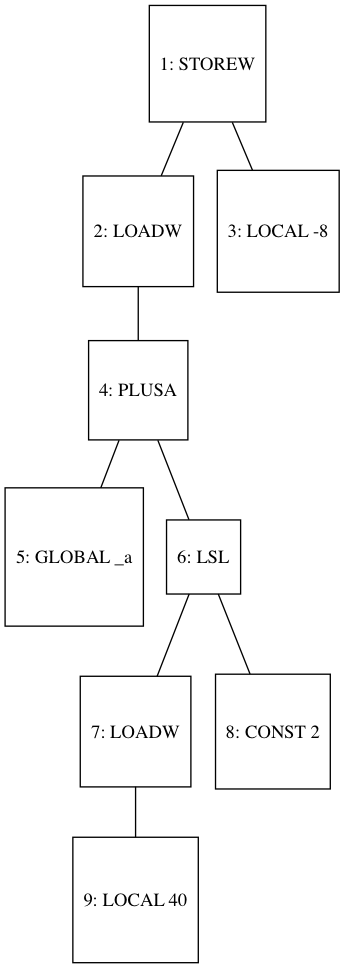
\includegraphics[width=.7\textwidth]{ex1.png}
\end{minipage}
\begin{minipage}[c]{.5\textwidth}
\begin{tabular}{|c|c|c|c|}

\hline
Node $i$ & Symbol $S$ & Rules & $d_i^S$ \\
\hline
1 & reg & & 0 \\
\hline
1 & rand & 10 & 0 \\
\hline
1 & addr & 14 & 0 \\
\hline
1 & stmt & 15 & \underline{28} \\
\hline

2 & reg & 4 & 14\\
\hline
2 & rand & 10 & 14\\
\hline
2 & addr & 14 & 14\\
\hline
2 & stmt & & 0 \\
\hline

3 & reg & 2 & 1\\
\hline
3 & rand & 10 & 1\\
\hline
3 & addr & 11, 14 & 2\\
\hline
3 & stmt & & 0 \\
\hline

4 & reg & 5 & 8\\
\hline
4 & rand & 10 & 8\\
\hline
4 & addr & 12, 13, 14& 14 \\
\hline
4 & stmt & & 0 \\

\hline
5 & reg & 3 & 1\\
\hline
5 & rand & 10 & 1\\
\hline
5 & addr & 14 & 1\\
\hline
5 & stmt & & 0 \\
\hline

6 & reg & 6 & 4\\
\hline
6 & rand & 8, 9, 10& 8\\
\hline
6 & addr & 14 & 4 \\
\hline
6 & stmt & & 0 \\
\hline

7 & reg & 4 & 2 \\
\hline
7 & rand & 10 & 2 \\
\hline
7 & addr & 14 & 2 \\
\hline
7 & stmt & & 0 \\
\hline

8 & reg & 1 & 1 \\
\hline
8 & rand & 7, 10 & 2 \\
\hline
8 & addr & 14 & 1\\
\hline
8 & stmt & & 0 \\
\hline

9 & reg & 2 & 1 \\
\hline
9 & rand & 10 & 1 \\
\hline
9 & addr & 11, 14& 2\\
\hline
9 & stmt & & 0 \\
\hline
\end{tabular}
\end{minipage}
So the answer is that there are 28 different tilings. \\

By inspecting all 28 trees, I've found that the shortest code is precisely the one in the notes:

\begin{lstlisting}{language=arm}
ldr r0, =_a
ldr r1, [fp, #40]
lsl r1, r1, #2
ldr r0, [r0, r1]
str r0, [fp, #-8]
\end{lstlisting}

And that the worst code is the one that uses the least specific rule at each possible choice (i.e. splits each node into its own tile), and that stores all temporary values in registers:

\begin{lstlisting}{language=arm}
ldr r0, [fp, #40]
ldr r1, [r0]
mov r2, #2
lsl r3, r1, r2
ldr r4, =_a
add r4, r4, r3
ldr r5, [r4]
ldr r6, [fp, #-8]
str r6, r0
\end{lstlisting}

This is almost the "bad" code from the notes, just that instead of directly computing \texttt{lsl r3, r1, \#2}, we first move \texttt{\#2} into a register and then compute this.

Assume pointers are 4 bytes and aligned to 4 bytes, and integers are 4 bytes and aligned to 4 bytes. \\
The record layout will be thus:
\begin{itemize}
\item 4 bytes for \texttt{data}
\item 4 bytes for \texttt{next}
\end{itemize}
and the record will be 4 byte aligned. \\

Suppose that the stack layout is thus:

\begin{itemize}
\item at fp - 8, the second local variable byte (supposijng it is 4 bytes long)
\item at fp - 4, the first local variable (supposing it is 4 bytes long)
\item at fp, the dynamic link
\item at fp + 4, the return address
\item at fp + 8, the beginning of the procedure currenty being run
\item at fp + 12, the static link
\item at fp + 16, the first argument
\item at fp + 20, the second argument
\item ...
\end{itemize}

The following is a Keiko instruction sequence that implements the given statements:

\asmenv{
    \asmr{Instruction}{Stack after instruction}
    \asmr{LOCAL -8}{\&s}
    \asmr{LOADW}{s}
    \asmr{LOCAL -4}{s; \&q}
    \asmr{LOADW}{s; q}
    \asmr{LOADW}{s; q$\uparrow$.data}
    \asmr{PLUS}{s + q$\uparrow$.data}
    \asmr{LOCAL -8}{s + q$\uparrow$.data; \&s}
    \asmr{STOREW}{}
    \asmr{LOCAL -4}{\&q}
    \asmr{LOADW}{q}
    \asmr{CONST 4}{q; 4}
    \asmr{OFFSET}{q + 4}
    \asmr{LOADW}{q$\uparrow$.next}
    \asmr{LOCAL -4}{q$\uparrow$.next; \&q}
    \asmr{STOREW}{}
}

The associated trees are found in diagram 2.

\section{}
Suppose x is at offset -4 from the frame pointer and y is at offset -8 from the frame pointer. \\
Code without movm:

\begin{lstlisting}
ldr r0, [fp, #-8]
str r0, [fp, #-4]
\end{lstlisting}

Code with movm:

\begin{lstlisting}
sub r0, fp, #8
sub r1, fp, #4
movm [r1], [r2]
\end{lstlisting}

So under the assumptions given, the code with movm is 50\% worse than the code without it.

\section{}
Suppose x and y are local pointers to pointers to integers, again at offests -4 and -8, and we want to compile \texttt{!!x := !!y}.
Code without movm:

\begin{lstlisting}
ldr r0, [fp, #-8]
ldr r1, [fp, #-4]
ldr r1, [r1]
str r1, [r0]
\end{lstlisting}

Code with movm:

\begin{lstlisting}
ldr r0, [fp, #-8]
ldr r1, [fp, #-4]
movm [r1], [r0]
\end{lstlisting}

\section{}


\section{Problem 8}

An abstract syntax that would 

\begin{lstlisting}[language=Ml]
type expr = IfExpr of expr * expr * expr
\end{lstlisting}

To add this to an Ocamlyacc grammar, take the grammar from lab 1 and replace the rules for $expr$ with:
\begin{lstlisting}[language=Ml]
expr :
    IF expr THEN expr ELSE expr { IfExpr ( $2, $4, $6 ) }
    | ifless_expr               { $1 }

ifless_expr :
    simple                     { $1 }
    | ifless_expr RELOP simple { Binop ($2, $1, $3) } 

\end{lstlisting}

This way of doing things makes this \texttt{if then else} construct have the highest possible precedence (i.e. \texttt{if e then e else e + if e then e else e} is interpreted as \texttt{if e then e else (e + if e then e else e)}).

\subsection{b}

To enhance gen\_expr to deal with this, simply add the following case:

\begin{lstlisting}[language=Ml]

let rec gen_expr = (* all the previous cases *)
    | IfExpr (c, e1, e2) -> 
        let lab1 = label () and lab2 = label () and lab3 = label () in
        SEQ [gen_cond c lab1 lab2 ;
            LABEL lab1 ; gen_expr e1 ; JUMP lab3 ;
            LABEL lab2 ; gen_expr e2 ; LABEL lab3 ]
\end{lstlisting}

Also, make it so that gen\_expr and gen\_cond can mutually recurse, as follows:

\begin{lstlisting}[language=Ml]

let rec gen_expr = (* ... *)
    and gen_cond = (* ... *)

\end{lstlisting}

\subsection{c}

The code generated by this is:

\ASMEnv{
\ASMRow{LDGW \_i}{}
\ASMRow{CONST 0}{}
\ASMRow{JGEQ L4}{}
\ASMRow{JUMP L5}{}
\ASMRow{LABEL L4}{}
\ASMRow{LDGW \_a}{}
\ASMRow{LDGW \_i}{}
\ASMRow{OFFSET}{}
\ASMRow{LOADW}{}
\ASMRow{LDGW \_x}{}
\ASMRow{JGT L1}{}
\ASMRow{JUMP L6}{}
\ASMRow{LABEL L5}{}
\ASMRow{CONST 0}{}
\ASMRow{LABEL L6}{}
\ASMRow{CONST 0}{}
\ASMRow{JNEQ L1}{}
\ASMRow{JUMP L2}{}
\ASMRow{LABEL L1}{}
\ASMRow{LDGW \_i}{}
\ASMRow{CONST 1}{}
\ASMRow{PLUS}{}
\ASMRow{STGW \_i}{}
\ASMRow{JUMP L3}{}
\ASMRow{LABEL L2}{}
\ASMRow{LABEL L3}{}
}

Some rules that would partially fix this code are:

\texttt{JGT a; JUMP b ; LABEL a} $\rightarrow$ \texttt{JLT b} \textit{with similar rules for other conditional jumps, assuming that a is not used elsewhere} \\
\texttt{LABEL a; LABEL b} $\rightarrow$ \texttt{LABEL a} \textit{substituting a for b everywhere else} \\
\texttt{JUMP a; LABEL a} $\rightarrow$ \texttt{LABEL a} \\

Applying these leads to:

\ASMEnv{
\ASMRow{LDGW \_i}{}
\ASMRow{CONST 0}{}
\ASMRow{JLT L5}{}
\ASMRow{LDGW \_a}{}
\ASMRow{LDGW \_i}{}
\ASMRow{OFFSET}{}
\ASMRow{LOADW}{}
\ASMRow{LDGW \_x}{}
\ASMRow{JGT L1}{}
\ASMRow{JUMP L6}{}
\ASMRow{LABEL L5}{}
\ASMRow{CONST 0}{}
\ASMRow{LABEL L6}{}
\ASMRow{CONST 0}{}
\ASMRow{JNEQ L1}{}
\ASMRow{JUMP L3}{}
\ASMRow{LABEL L1}{}
\ASMRow{LDGW \_i}{}
\ASMRow{CONST 1}{}
\ASMRow{PLUS}{}
\ASMRow{STGW \_i}{}
\ASMRow{LABEL L3}{}
}

This is still not quite as good as the code generated by the native and, as this code still has an annoying comparison to $0$ (as a conditional on an if expression first evaluates the expression then compares the result to $0$). I am not sure how to fix this.

\section{Problem 3.1}

\ASMEnv{
\ASMRow{LDGW s}{}
\ASMRow{LDGW q}{}
\ASMRow{LOADW}{}
\ASMRow{PLUS}{}
\ASMRow{STGW s}{}
\ASMRow{LDGW q}{}
\ASMRow{OFFSET 4}{}
\ASMRow{LOADW}{}
\ASMRow{STGW q}{}
}

\section{Problem 3.2}

This design change has several parts that need to be treated:
\begin{itemize}
\item First, we need to add new tokens \texttt{LOCAL} (matching only \texttt{local}), and \texttt{IN} (matching only \texttt{in}).
\item Second, we need to add statements of type \texttt{LocalDecl of decls list * stmt} to the abstract syntax. No change is needed to type \texttt{program}.
\item Third, we need to add a new rule to the grammar: \texttt{stmt: LOCAL decls IN stmt END \{LocalDecl($2, $4)\}}.
\item Fourth, we add a new scoping check (i.e. we check that all variables are only used in blocks where they are declared).
\item
\begin{minipage}[t]{\linewidth}
    Now, we make an intermediate translation, with the eventual goal of transforming local statements into equivalent global declarations.  First, dealing with name conflicts (i.e. redeclaring a variable in a more deeply nested block). I think the easiest and cleanest way to deal with scope is with name mangling -- i.e. we have a translation step that transforms:
\begin{lstlisting}[language=pascal]
local var y : t;
in
    stmt[y]
end
\end{lstlisting}

into
\begin{lstlisting}[language=pascal]
local var mangledy : t;
in
    stmt[mangledy]
end
\end{lstlisting}
where stmt[t] is notation for a statement that contains some variable name t, stmt[u] means that same statement just with all unbound appearences of t replaced by u, and mangledy is some string that is distinct from all other variable names in the program (one such mangling scheme would be to append the number of \texttt{local} blocks already processed when the variable is declared, or to append a long random string). By unbound I mean that appearences within another \texttt{local} block of the same variable, where the variable was re-declared in that local block, do not count. Note that this transformation does not change the semantics of the program.
\end{minipage}
\item After applying the previous translation, note that since all the variables now have distinct names, we could just have well as declared all of them globally. This suggests what we must now do; more precisely, move all declarations from \texttt{local} blocks into the global declaration.
\item Now, as we know that variables are used only in the correct scopes, and also as the syntax tree has the same form as a syntax tree without local blocks, we can simply use the old checking, annotating and code generating functions.
\end{itemize}

% We can implement these in a single pass function \texttt{translate}, defined below
% 
% 
% \begin{lstlisting}[language=Ml]
% 
% open List
% open List.Assoc
% 
% let translate (Program (decls, stmt)) =
%     let local_counter = ref 0 in
%     and mangle str = str ^ string_of_int !local_counter
%     and mangle_decl (Decl (names, pt))
%         = Decl (map (function n -> { x_name = mangle n.x_name
%                                    ; n.x_line
%                                    ; n.x_def
%                                    })
%                     , pt)
%     and mangle_decls = map mangle_decl
%     and change_context context decls =
%         let all_names = map (fun n -> n.x_name) (concat (fst (split decls)))
%         and context_diff = map (fun x -> (x, mangle x)) all_names in
%         foldright add context_diff context
%     and apply_context_to_string context str =
%         if mem str context then find str context else str
%     and apply_context_to_name n str =
%         { x_name = apply_context_to_string context n.x_name
%         ; x_line = n.x_line
%         ; x_def = n.x_def
%         } in
%     (* tr_stmt takes a context : list (string * string) of name changes,
%      * and a stmt and returns a list of declarations to be included at the
%      * beginning of the block and the new statement, as a pair*)
%     (* tr_expr tkaes a context and an expr and returns the
%      * expr with variables names mangled w.r.t. the context *)
%     let rec tr_expr context
%         = function
%         Variable x -> apply_context_to_name x context
%         | Constant x -> Constant x
%         | Monop (w, e1) -> Monop (w, tr_expr context e1)
%         | Binop (w, e1, e2) -> Binop (w, tr_expr context e1
%                                      , tr_expr context e2) in
%     let rec tr_stmt context
%         = function
%         Local (decls, stmt) ->
%             let new_context = change_context context decls
%             and mangled_decls = mangle_decls decls
%             and (ret_decls, ret_stmt) = tr_stmt new_context stmt
%             in (mangled_decls @ ret_decls, ret_stmt)
%         | (* very many tedious repetitive cases, all of which
%            * boil down to simply recursivly applying tr_stmt
%            * or tr_expr ; some examples included for illustration *)
%         | IfStmt (test, thenpt, elsept) ->
%             let test_tr = tr_expr test
%             and (thenpt_decls, thenpt_tr) = tr_stmt thenpt
%             and (elsept_decls, elsept_tr) = tr_stmt elsept
%             in (thenpt_decls @ elsept_decls
%                , IfStmt(test_tr, thenpt_tr, elsept_tr))
%         | WhileStmt (test, body) ->
%             let test_tr = tr_expr test
%             and (body_decls, body_tr) = tr_stmt body
%             in (body_decls, WhileStmt(test_tr, body_tr)) in
%     let (newdecls, newstmt) = tr_stmt [] stmt in
%         Program (decls @ newdecls, newstmt)
% 
% \end{lstlisting}

\section{Problem 3.4}
It is impossible to be able to do this with perfect accuracy at compile-time, because the variables that are initialised at any time might depend on information known only at run-time (such as user-input). I would err on the side of being more restrictive rather than less restrictive -- forcing variables to always have some though-out assigned value before use makes programmers think about these edge cases, which eliminates a whole class of bugs. Thus I would enforce a rule that a variable must be assigned before use no matter what the execution path through the code. The most difficult control structure to deal with is \texttt{exit}, as only these break normal control flow. A function that checks this property follows:

\begin{lstlisting}[language=Ml]

let intersect2 xs ys = filter (fun x -> mem x xs) ys
let intersect (xs :: xss) = fold_right intersect2 xss xs 

let has_exit = function
    Seq (x :: xs) -> has_exit x || has_exit (Seq xs)
    | Exit -> true
    | IfStmt(e, ifpt, elsept) -> has_exit ifpt || has_exit elsept
    | WhileStmt(test, body) -> has_exit body
    | RepeatStmt(body, test) -> has_exit body
    | LoopStmt body -> false
    | CaseStmt (switch, cases, default) ->
        has_exit default || exists has_exit (map snd cases)
    | _ -> false

let will_exit = function
    Seq (x :: xs) -> will_exit x || will_exit (Seq xs)
    | Exit -> true
    | IfStmt(e, ifpt, elsept) -> will_exit ifpt && will_exit elsept
    | WhileStmt _ -> false
    | RepeatStmt (body, test) -> will_exit body
    | LoopStmt body -> false
    | CaseStmt (switch, cases, default) ->
        will_exit default && for_all will_exit (map snd cases)
    | _ -> false

(* f takes an expression and returns the variables it uses
 * g takes a statement and returns a tuple: the variables it
 * needs to be initialised prior, and the variables it
 * certainly initialises *)
let test_stmt = 
    let rec f = function
        Constant _ -> []
        | Variable x -> [x.x_lab]
        | Monop (_, e) -> f e
        | Binop (_, e1, e2) -> f e1 @ f e2 in
    let rec g = function
        Skip -> ([], [])
        | Seq (x :: xs) ->
            (* A sequence needs everything that the first part needs,
             * together with everything the second part needs that is
             * not defined in the first part.
             * A sequence defines everything that the first or second
             * part defines
             * SPECIAL CASE: if the first thing will exit, then ignore
             * the rest. If the first thing might exit, then we
             * must take into account the entire Seq for needs,
             * and only the first part for things it defines *)
            let (usedl, defsl) = g x
            and (usedr, defsr) = g (Seq xs)
            and used = usedl @ (filter (fun x -> not (mem x defsl)) usedr)
            and defs = defsl @ defsr
            in if will_exit x then (usedl, defsl)
            else if has_exit x then (used, defsl)
            else (used, defs)
        | Seq [] -> ([], [])
        | Assign (v, e) -> (f e, [v.x_lab])
        | Print e -> (f e, [])
        | Newline -> ([], [])
        | IfStmt (test, thenpt, elsept) ->
            (* An if statement needs everything any of its clauses
             * needs, and defines only what both of its clauses
             * defines *)
            let used1 = f test
            and (used2, defs2) = g thenpt
            and (used3, defs3) = g elsept
            in (used1 @ used2 @ used3
               , intersect2 defs2 def3)
        | WhileStmt (test, body) ->
            (* a while statement needs everything its test or
             * body might need, and defines nothing (as the body
             * might not even be run *)
            let used1 = f test
            and (used2, _) = g body
            in (used1 @ used2, [])
        | RepeatStmt (body, test) ->
            (* a repeat statement is like a while, just that
             * it defines everything its body defines, since
             * the body is guaranteed to be run *)
            let used1 = f test
            and (used2, defs) = g body
            in (used1 @ used2, defs)
        | ExitStmt -> ([], [])
        | LoopStmt body ->
            (* A loop statement needs everything its body needs,
             * and defines what it's body defines *)
             g body
        | CaseStmt (switch, cases, default) ->
            (* A case statement needs everything any of its
             * body or switch needs, and defines whatever
             * all of the cases defines for sure *)
            let used1 = f switch
            and used2 = concat (map fst (map g (map snd cases)))
            and defs2 = map snd (map g (map snd cases))
            and (used3, defs3) = g default
            in (used1 @ used2 @ used3, intersect (defs3 :: defs2))
    in function x -> length (fst (g x)) == 0

\end{lstlisting}


\end{document}
